\ifx\allfiles\undefined
\documentclass[12pt, a4paper, oneside, UTF8]{ctexbook}
\def\path{../config}
\input{../config/_config}
\begin{document}
% \input{../config/cover}
\else
\fi

\chapter{概率论部分}

\section{事件与概率论}
% 第一章 题型一
\subsection{事件的关系、运算与概率的性质}
\begin{enumerate}
    \item 事件:样本点的\textbf{集合} 
    \item 事件的关系(3+1): 包含,互斥,对立 + 独立 
    \item 事件的运算(3个):交,并,补 
\end{enumerate}
\begin{remark}(事件的运算律)
    \item [(1)]\quad 交换律 \qquad $A\cup B = B\cup A, AB=BA$
    \item [(2)]\quad 结合律 \qquad $A\cup(B\cup C)=(A\cup B)\cup A, A(BC)=(AB)C$
    \item [(3)]\quad 分配律 \qquad $A\cup(BC)=(A\cup B)(A\cup C), A(B\cup C)=(AB)\cup(AC)$
    \item [(4)]\quad 摩根律 \qquad $\overline{A\cup B}=\bar{A}\bar{B},\overline(AB)=\bar{A}\cup\bar{B}$
    \item [(5)]\quad 吸收律 \qquad $A\cup(AB)=A,A(A\cup B)=A$
\end{remark}

\begin{enumerate}[label=\arabic*.]
    % 例题1.1
    \item 设$A,B$为随机事件,且$P(A)=P(B)=\frac{1}{2}$,$P(A\cup B)=1$,则
    \begin{align*}
        (A)\ A\cup B=\Omega \quad (B)\ AB=\varnothing \quad (C)\ P(\bar{A}\cup\bar{B})=1 \quad (D)\ P(A-B)=0
    \end{align*}

    \begin{solution}
    由加法公式
    $P(A\cup B) = P(A) + P(B) - P(AB)\implies P(AB) = 0$ 
    \newline
    注意由概率并不能推断事件,所以(A)(B)均不正确 \\
    对于(C)选项 $P(\bar{A}\cup\bar{B}) = 1 - P(\overline{AB}) = 1$ 正确 \\
    对于(D)选项,由减法公式 $P(A-B) = P(A) - P(AB) = \frac{1}{2}$
    \end{solution}
    
    \begin{tcolorbox}[title=总结]
        (1)必然事件发生的概率为1,但概率为一的事件不一定是必然事件  \\
        (2)不可能事件发生的概率为0,但概率为零的事件不一定是不可能事件 \\
        这两个结论考虑\textbf{连续型随机变量}即可
    \end{tcolorbox}

    % 例题1.2
    \item (2020,数一、三)设$A,B,C$为随机事件,且$P(A)=P(B)=P(C)=\frac{1}{4}$,$P(AB)=0$,$P(AC)=P(BC)=\frac{1}{12}$,则$A,B,C$只有一个事件发生的概率为
    \begin{align*}
        (A)\ \frac{3}{4} \quad (B)\ \frac{2}{3} \quad (C)\ \frac{1}{2} \quad (D)\ \frac{5}{12}
    \end{align*}
    \begin{solution}
    这种题一般考虑Venn图,比用公式展开简单很多
    \begin{center}
    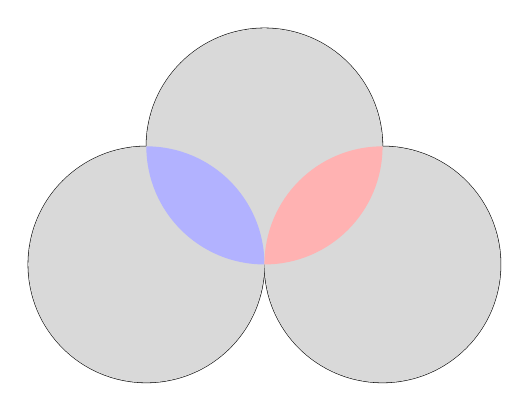
\begin{tikzpicture}[scale=1.5]

        % 定义三个圆的位置和大小
        \draw (0,0) circle (1cm) node[above left] {A};
        \draw (2,0) circle (1cm) node[above right] {B};
        \draw (1,1) circle (1cm) node[above] {C};

        % 填充颜色(可选)
        \fill[gray!30] (0,0) circle (1cm); % A 的独有部分
        \fill[gray!30] (2,0) circle (1cm); % B 的独有部分
        \fill[gray!30] (1,1) circle (1cm); % C 的独有部分

        % 填充 AC 重叠部分(A 和 C 的交集)
        \begin{scope}
            \clip (0,0) circle (1cm);
            \fill[blue!30] (1,1) circle (1cm);
        \end{scope}

        % 填充 BC 重叠部分(B 和 C 的交集)
        \begin{scope}
            \clip (2,0) circle (1cm);
            \fill[red!30] (1,1) circle (1cm);
        \end{scope}

        % 确保 AC 和 BC 重叠部分面积相等(通过对称性保证)
    \end{tikzpicture}
    \end{center}
    则只有一个事件发生的概率为
        $(\frac{1}{4} - \frac{1}{12})\times 2 + \frac{1}{4} 
        - 2\times \frac{1}{12} = \frac{5}{12}$
    \end{solution}
    
    % 例题1.3
    \item 设随机事件$A,B$满足$AB=\bar{A}\bar{B}$,且$0<P(A)<1$,$0<P(B)<1$,则$P(A|\bar{B})+P(B|\bar{A})=\_\_\_\_\_$
    
    \begin{solution}
    根据结论,有$A,B$互斥,则$P(A|\bar{B})=P(B|\bar{A})=1$
    \end{solution}

    \begin{corollary}
        若$AB=\bar{A}\bar{B}$,则$A,B$必然对立
        \begin{proof}
            \begin{align*}
                &AB =\bar{A}\bar{B} \\
                &\iff AB\cup \bar{A}B =\bar{A}\bar{B}\cup \bar{A}B \\
                &\iff (A\cup \bar{A})B = \bar{A}(\bar{B}\cup B) \\
                &\iff B = \bar{A}
            \end{align*}
        \end{proof}
    \end{corollary}

    % 例题 1.4
    \item 设随机事件$A,B,C$两两独立,满足$ABC=\varnothing$,且$P(A)=P(B)=P(C)$,$A,B,C$至少有一个发生的概率为$\frac{9}{16}$,则$P(A)=$
    
    \begin{solution}
    由题意有$P(A\cup B\cup C) = \frac{9}{16}$,由加法公式与独立性有
    \begin{align*}
        P(A\cup B\cup C) 
        &= P(A) + P(B) + P(C) - P(A)P(B) \\
        &- P(A)P(C) - P(B)P(C) - P(A)P(B)P(C)
    \end{align*}
    由$P(A)=P(B)=P(C)$,上式化为$3P(A)-3P(A)^2 = \frac{9}{16}\implies P(A)=\frac{1}{4}\text{或}P(A)=\frac{3}{4}$,
    显然$P(A)\neq \frac{3}{4} > P(A\cup B\cup C)$,故$P(A)=\frac{1}{4}$
    \end{solution}
    
    % 例题 1.5
    \item 设$A,B$为随机事件,且$P(A)=\frac{2}{3}$,$P(B)=\frac{1}{2}$,则$P(A|B)+P(B|A)$的最大值为\_\_\_\_,最小值为\_\_\_\_.
    
    \begin{solution}
    关于概率的不等式基于如下事实,对于任意一个概率其值均位于$[0,1]$之间,事件AB的和事件不可能小于单独A,B发生概率之和,事件AB的积事件不可能大于
    任意一个事件单独发生的概率.
    \[
    P(A)+P(B) - 1<=P(AB) \leq \min{(P(A),P(B))}  \leq P(A) + P(B) \leq P(A\cup B) 
    \]
    \end{solution}
\end{enumerate}

\subsection{三大概型的计算}
\begin{remark}
    三大概率模型
    \item 经典概型 -- 有限个等可能的样本点,\textbf{排列组合问题}
    \item 几何概型 -- 使用几何参数度量概率,比如说长度,面积,体积等
    \item 伯努利概型 -- 独立重复试验每次成功的概率为$p$,不成功的概率为($1-p$)
\end{remark}
\begin{enumerate}[label=\arabic*.,start=6]
    % 例题 1.6
    \item (2016,数三)设袋中有红、白、黑球各1个,从中\textbf{有放回地}取球,每次取1个,直到三种颜色的球都取到为止,则取球次数恰好为4的概率为
    
    \begin{solution}
    (古典概型) 
    \[\frac{\binom{3}{1}\binom{2}{1}\binom{2}{3}}{3^4}=\frac{2}{9}\]
    首先从3个颜色中选择一个为第四次抽的颜色,再从剩下两个颜色中选择一个为出现两次的颜色,在选择该颜色抽出的次序.
    \end{solution}
    % 例题 1.7
    \item 在区间$(0,a)$中随机地取两个数,则两数之积小于$\frac{a^2}{4}$的概率为
    
    \begin{solution}
    (几何概型)
    \[
    \frac{\frac{a}{4}\cdot a + \int_{\frac{a}{4}}^{a}\frac{a^2}{4x}dx}{a^2} = \frac{1}{4} + \frac{1}{2}\ln{2}
    \]
    \end{solution}
    % 例题 1.8
    \item 设独立重复的试验每次成功的概率为$p$,则第5次成功之前至多2次失败的概率为
    
    \begin{solution}
    失败零次--$p^5$,失败一次--$\binom{1}{5}p^4(1-p)p$,失败两次--$\binom{2}{6}p^4(1-p)^2p$ \\
    故第5次成功之前至多2次失败的概率为
    \[
    p^5 + \binom{1}{5}p^4(1-p)p + \binom{2}{6}p^4(1-p)^2p
    \]
    \end{solution}
\end{enumerate}

\subsection{三大概率公式的计算}
\begin{remark}
    三大概率公式
    \item 条件概率公式\qquad $P(A\mid B)=\frac{P(AB)}{P(B)}$ \\
    推论 $P(AB)=P(B)P(A\mid B), P(A_1A_2\ldots A_n)=P(A_1)P(A_2\mid P(A_1))P(A_3|P(A_1A_2))\ldots$
    \item 全概率公式\qquad $P(A)=\sum_{i=1}^{n}P(AB_i)=\sum_{i=1}^{n}P(B_i)P(A\mid B_i)$
    \item 贝叶斯公式\qquad $P(B_j\mid A)=\frac{P(B_j)P(A\mid B_j)}{\sum_{i=1}^{n}P(B_i)P(A\mid B_i)}$
\end{remark}

\begin{enumerate}[label=\arabic*.,start=9]
    % 例题 1.9
    \item 设$A,B$为随机事件,且$P(A\cup B)=0.6$,$P(B|\bar{A})=0.2$,则$P(A)=\_\_\_\_$
    
    \begin{solution}
    \[P(A\cup B)=P(A) + P(B) - P(AB) = 0.6, P(B\mid\bar{A})=\frac{P(B)-P(AB)}{1-P(A)} = 0.2\]
    联立有
    \[\frac{0.6 - P(A)}{1 - P(A)} = 0.2\],则$P(A)=0.5$
    \end{solution}
    
    % 例题 1.10
    \item  (2018,数一)设随机事件$A$与$B$相互独立,$A$与$C$相互独立,满足$BC=\varnothing$,且
    \begin{align*}
        P(A)=P(B)=\frac{1}{2},\quad P(AC|AB\cup C)=\frac{1}{4},
    \end{align*}
    则$P(C)=$\_\_\_\_.
    
    \begin{solution}
    \begin{align*}
        P(AC|AB\cup C)
        &= \frac{P(AC)}{P(AB\cup C)} \\
        &=\frac{P(A)P(C)}{P(AB)+P(C)} \\
        &=\frac{\frac{1}{2}P(C)}{\frac{1}{4} + P(C)} = \frac{1}{4}
    \end{align*}
    则$P(C)=\frac{1}{4}$
    \end{solution}
    
    % 例题 1.11
    \item  (2003,数一)设甲、乙两箱装有同种产品,其中甲箱装有3件合格品和3件次品,乙箱装有3件合格品。从甲箱中任取3件产品放入乙箱,
    \begin{enumerate}[label=(\roman*)]
        \item[(1)] 求乙箱中次品件数$X$的数学期望;
        \item[(2)] 求从乙箱中任取一件产品是次品的概率.
    \end{enumerate}

    \begin{solution}(作为小题来考还可以)
    \item [方法一] 
    \item{(1)} 对于数字特征的题目,先求概率分布再说,由于$P(X=k)=\frac{C_{3}^{k}C_{3-k}^{k}}{C_{6}^{3}}$
    \begin{center}
        \begin{tabular}{|c|c|c|c|c|}
        \hline
        $ x $ & 0 & 1 & 2 & 3 \\ \hline
        $ P(x) $ & $ \frac{1}{20} $ & $ \frac{9}{20} $ & $ \frac{9}{20} $ & $ \frac{1}{20} $ \\ \hline
        \end{tabular}
    \end{center}
    则所求数学期望$EX=\frac{9}{20} + 2\times \frac{9}{20} + \frac{3}{20} = \frac{3}{2}$
    \item [(2)] 
    \begin{align*}
        P(A) &=\sum_{k=0}^{3}P(X=k)P(A\mid x=k)  \\
        &= \frac{1}{20} \times 0 + \frac{9}{20}\times\frac{1}{6} 
        + \frac{9}{20}\times\frac{2}{6} + \frac{1}{20}\times \frac{3}{6}  \\
        &= \frac{1}{4}
    \end{align*}

    \item [方法二:超几何分布]  
    \item [(1)] $X\sim H(N, M, n), N = 6, M = 3, n = 3$, 则$EX=\frac{nM}{N}=\frac{3}{2}$
    \item [(2)]
    \begin{align*}
        P(A) &=\sum_{k=0}^{3}P(X=k)P(A\mid x=k) \\
        &= \sum_{k=0}^{3}P(X=k) \frac{k}{6} \\
        &= \frac{1}{6}\sum_{k=0}^{3}P(X=k)k \\
        &= \frac{1}{6}EX \\
        &= \frac{1}{4}
    \end{align*}
    \end{solution}
\end{enumerate}

\subsection{事件独立的判定}

\begin{remark}(事件独立的充要条件)
\begin{align*}
        & P(AB) = P(A)P(B) \\
        & \iff P(A\mid B) = P(A) \\
        & \iff P(A\mid \bar{B}) = P(A) \iff P(A\mid B) = P(A\mid \bar{B}) \quad (0 < P(B) < 1) \\
        & \iff A \text{ 与 } \bar{B}, \text{ 或 } \bar{A} \text{ 与 } B, \text{ 或 } \bar{A} \text{ 与 } \bar{B} \text{ 相互独立} \\
        & \iff P(A\mid B) + P(\bar{A} \mid \bar{B}) = 1, \quad 0 < P(B) < 1
\end{align*}
\end{remark}

\begin{enumerate}[label=\arabic*.,start=12]
    % 例题 1.12
    \item  设$A,B$为随机事件,且$0<P(A)<1$,则 \\
        (A)\ 若$A\supset B$,则$A,B$一定不相互独立 \\
        (B)\ 若$B\supset A$,则$A,B$一定不相互独立 \\
        (C)\ 若$AB=\varnothing$,则$A,B$一定不相互独立 \\
        (D)\ 若$A=\bar{B}$,则$A,B$一定不相互独立
    
    \begin{solution}
    
    \end{solution}
    
    % 例题 1.13
    \item  设$A,B,C$为随机事件,$A$与$B$相互独立,且$P(C)=0$,则$\bar{A},\bar{B},\bar{C}$
    \newline
    \text{(A)}相互独立\qquad \text{(B)}两两独立,但不一定相互独立 \\
    \text{(C)}不一定两两独立\qquad \text{(D)}一定不两两独立
    \begin{solution}
    【详解】
    \end{solution}
\end{enumerate}

\newpage

\section{一维随机变量}

\subsection{分布函数的判定与计算}

\begin{enumerate}[label=\arabic*.]
    % 例题 2.1
    \item 设随机变量$X$的分布函数为$F(x)$,$a,b$为任意常数,则下列一定不是分布函数的是
    \begin{align*}
        (A)\ F(ax+b) \quad (B)\ F(x^2+b) \quad (C)\ F(x^3+b) \quad (D)\ 1-F(-x)
    \end{align*}
    
    \begin{solution}
    【详解】
    \end{solution}
    
    \item 设随机变量$X$的概率密度为
    \begin{align*}
        f(x)=\begin{cases}
            1-|x|, & |x|<1 \\
            0, & \text{其他}
        \end{cases}
    \end{align*}
    则$X$的分布函数$F(x)=$?,$P\{-2<X<\frac{1}{4}\}=$?.
    
    \begin{solution}
    【详解】
    \end{solution}
\end{enumerate}

\subsection{概率密度的判定与计算}

\begin{enumerate}[label=\arabic*.,start=3]
    \item 设随机变量$X$的概率密度为$f(x)$,则下列必为概率密度的是
    \begin{align*}
        (A)\ f(-x+1) \quad (B)\ f(2x-1) \quad (C)\ f(-2x+1) \quad (D)\ f\left(\frac{1}{2}x-1\right)
    \end{align*}
    
    \begin{solution}
    【详解】
    \end{solution}
    
    \item (2011,数一、三)设$F_1(x),F_2(x)$为分布函数,对应的概率密度$f_1(x),f_2(x)$为连续函数,则下列必为概率密度的是
    \begin{align*}
        (A)\ f_1(x)f_2(x) \quad (B)\ 2f_2(x)F_1(x) \quad (C)\ f_1(x)F_2(x) \quad (D)\ f_1(x)F_2(x)+f_2(x)F_1(x)
    \end{align*}
    
    \begin{solution}
    【详解】
    \end{solution}
    
    \item (2000,三)设随机变量$X$的概率密度为
    \begin{align*}
        f(x)=\begin{cases}
            \frac{1}{3}, & x\in[0,1] \\
            \frac{2}{9}, & x\in[3,6] \\
            0, & \text{其他}
        \end{cases}
    \end{align*}
    若$P\{X\geq k\}=\frac{2}{3}$,则$k$的取值范围是?.
    
    \begin{solution}
    【详解】
    \end{solution}
\end{enumerate}

\subsection{关于八大分布}

\begin{enumerate}[label=\arabic*.,start=6]
    \item 设随机变量$X$的概率分布为$P\{X=k\}=C\frac{\lambda^k}{k!}$,$k=1,2,\cdots$,则$C=$?.
    
    \begin{solution}
    【详解】
    \end{solution}
    
    \item 设随机变量$X$的概率密度为$f(x)=Ae^{-\frac{x^2}{2}+Bx}$,且$EX=DX$,则$A=$?,$B=$?.
    
    \begin{solution}
    【详解】
    \end{solution}
    
    \item (2004,数一、三)设随机变量$X\sim N(0,1)$,对给定的$\alpha(0<\alpha<1)$,数$u_\alpha$满足$P\{X>u_\alpha\}=\alpha$。若$P\{|X|<x\}=\alpha$,则$x$等于
    \begin{align*}
        (A)\ u_{\frac{\alpha}{2}} \quad (B)\ u_{1-\frac{\alpha}{2}} \quad (C)\ u_{\frac{1-\alpha}{2}} \quad (D)\ u_{1-\alpha}
    \end{align*}
    
    \begin{solution}
    【详解】
    \end{solution}
    
    \item 设随机变量$X\sim N(2,\sigma^2)$,且$P\{2<X<4\}=0.3$,则$P\{X<0\}=$?.
    
    \begin{solution}
    【详解】
    \end{solution}
    
    \item  设随机变量$X\sim N(\mu,\sigma^2)(\mu<0)$,$F(x)$为其分布函数,$a$为任意常数,则
    \begin{align*}
        (A)\ F(a)+F(-a)>1 \quad (B)\ F(a)+F(-a)=1 \\
        (C)\ F(a)+F(-a)<1 \quad (D)\ F(\mu+a)+F(\mu-a)=\frac{1}{2}
    \end{align*}
    
    \begin{solution}
    【详解】
    \end{solution}
    
    \item  设随机变量$X$与$Y$相互独立,均服从参数为1的指数分布,则$P\{1<\max\{X,Y\}<2\}=$?.
    
    \begin{solution}
    【详解】
    \end{solution}
    
    \item  设随机变量$X$与$Y$相互独立,均服从区间$[0,3]$上的均匀分布,则$P\{1<\min\{X,Y\}<2\}=$?.
    
    \begin{solution}
    【详解】
    \end{solution}
    
    \item  (2013,数一)设随机变量$Y\sim E(1)$,$a>0$,则$P\{Y\leq a+1|Y>a\}=$?.
    
    \begin{solution}
    【详解】
    \end{solution}
    
    \item  设随机变量$X\sim G(p)$,$m,n$为正整数,则$P\{X>m+n|X>m\}$
    \begin{align*}
        (A)\ 与m无关,与n有关,且随n的增大而减少 \\
        (B)\ 与m无关,与n有关,且随n的增大而增大 \\
        (C)\ 与n无关,与m有关,且随m的增大而减少 \\
        (D)\ 与n无关,与m有关,且随m的增大而增大
    \end{align*}
    
    \begin{solution}
    【详解】
    \end{solution}
\end{enumerate}

\subsection{求一维连续型随机变量函数的分布}

\begin{enumerate}[label=\arabic*.,start=15]
    \item  设随机变量$X\sim E(\lambda)$,则$Y=\min\{X,2\}$的分布函数
    \begin{align*}
        (A)\ 为连续函数 \quad (B)\ 为阶梯函数 \\
        (C)\ 至少有两个间断点 \quad (D)\ 恰好有一个间断点
    \end{align*}
    
    \begin{solution}
    【详解】
    \end{solution}
    
    \item  (2013,数一)设随机变量$X$的概率密度为
    \begin{align*}
        f(x)=\begin{cases}
            \frac{2x}{a^2}, & 0<x<a \\
            0, & \text{其他}
        \end{cases}
    \end{align*}
    $Y=\begin{cases}
        \frac{1}{3}X, & X\leq 1 \\
        X, & 1<X<2 \\
        1, & X\geq 2
    \end{cases}$
    \begin{enumerate}
        \item 求$Y$的分布函数;
        \item 求$P\{X\leq Y\}$.
    \end{enumerate}
    
    \begin{solution}
    【详解】
    \end{solution}
    
    \item  (2021,数一、三)在区间$(0,2)$上随机取一点,将该区间分成两段,较短一段的长度记为$X$,较长一段的长度记为$Y$。
    \begin{enumerate}
        \item 求$X$的概率密度;
        \item 求$Z=\frac{Y}{X}$的概率密度;
        \item 求$E\left(\frac{Y}{X}\right)$.
    \end{enumerate}
    
    \begin{solution}
    【详解】
    \end{solution}
\end{enumerate}

\section{二维随机变量}

\subsection{联合分布函数的计算}

\begin{enumerate}[label=\arabic*.]
    \item 设随机变量$X$与$Y$相互独立,$X\sim B(1,p)$,$Y\sim E(\lambda)$,则$(X,Y)$的联合分布函数$F(x,y)=$?.
    
    \begin{solution}
    【详解】
    \end{solution}
\end{enumerate}

\subsection{二维离散型随机变量分布的计算}

\begin{enumerate}[label=\arabic*.,start=2]
    \item 设随机变量$X$与$Y$相互独立,均服从参数为$p$的几何分布。
    \begin{enumerate}
        \item 求在$X+Y=n(n\geq 2)$的条件下,$X$的条件概率分布;
        \item 求$P\{X+Y\geq n\}(n\geq 2)$.
    \end{enumerate}
    
    \begin{solution}
    【详解】
    \end{solution}
\end{enumerate}

\subsection{二维连续型随机变量分布的计算}

\begin{enumerate}[label=\arabic*.,start=4]
    \item (2010,数一、三)设二维随机变量$(X,Y)$的概率密度为
    \begin{align*}
        f(x,y)=Ae^{-2x^2+2xy-y^2}, \quad -\infty<x<+\infty, -\infty<y<+\infty
    \end{align*}
    求常数$A$及条件概率密度$f_{Y|X}(y|x)$.
    
    \begin{solution}
    【详解】
    \end{solution}
    
    \item 设随机变量$X\sim U(0,1)$,在$X=x(0<x<1)$的条件下,随机变量$Y\sim U(x,1)$。
    \begin{enumerate}
        \item 求$(X,Y)$的联合概率密度;
        \item 求$(X,Y)$关于$Y$的边缘概率密度$f_Y(y)$;
        \item 求$P\{X+Y>1\}$.
    \end{enumerate}
    
    \begin{solution}
    【详解】
    \end{solution}
    
    \item 设二维随机变量$(X,Y)\sim N(1,2;1,4;-\frac{1}{2})$,且$P\{aX+bY\leq 1\}=\frac{1}{2}$,则$(a,b)$可以为
    \begin{align*}
        (A)\ \left(\frac{1}{2},-\frac{1}{4}\right) \quad (B)\ \left(\frac{1}{4},-\frac{1}{2}\right) \\
        (C)\ \left(-\frac{1}{4},\frac{1}{2}\right) \quad (D)\ \left(\frac{1}{2},\frac{1}{4}\right)
    \end{align*}
    
    \begin{solution}
    【详解】
    \end{solution}
    
    \item (2020,数三)设二维随机变量$(X,Y)\sim N(0,0;1,4;-\frac{1}{2})$,则下列随机变量服从标准正态分布且与$X$相互独立的是
    \begin{align*}
        (A)\ \frac{\sqrt{5}}{5}(X+Y) \quad (B)\ \frac{\sqrt{5}}{5}(X-Y) \\
        (C)\ \frac{\sqrt{3}}{3}(X+Y) \quad (D)\ \frac{\sqrt{3}}{3}(X-Y)
    \end{align*}
    
    \begin{solution}
    【详解】
    \end{solution}
    
    \item (2022,数一)设随机变量$X\sim N(0,1)$,在$X=x$的条件下,随机变量$Y\sim N(x,1)$,则$X$与$Y$的相关系数为
    \begin{align*}
        (A)\ \frac{1}{4} \quad (B)\ \frac{1}{2} \quad (C)\ \frac{\sqrt{3}}{3} \quad (D)\ \frac{\sqrt{2}}{2}
    \end{align*}
    
    \begin{solution}
    【详解】
    \end{solution}
\end{enumerate}

\subsection{求二维离散型随机变量函数的分布}

\begin{enumerate}[label=\arabic*.,start=12]
    \item 设随机变量$X$与$Y$相互独立,$X\sim P(\lambda_1)$,$Y\sim P(\lambda_2)$,求$Z=X+Y$的概率分布.
    
    \begin{solution}
    【详解】
    \end{solution}
\end{enumerate}

\subsection{求二维连续型随机变量函数的分布}

\begin{enumerate}[label=\arabic*.,start=13]
    \item 设二维随机变量$(X,Y)$的联合概率密度为
    \begin{align*}
        f(x,y)=\begin{cases}
            1, & 0<x<1,0<y<2x \\
            0, & \text{其他}
        \end{cases}
    \end{align*}
    求:
    \begin{enumerate}
        \item $(X,Y)$的联合分布函数$F(x,y)$;
        \item $(X,Y)$的边缘概率密度$f_X(x),f_Y(y)$;
        \item 条件概率密度$f_{X|Y}(x|y),f_{Y|X}(y|x)$;
        \item $P\left\{Y\leq \frac{1}{2}|X\leq \frac{1}{2}\right\}$,$P\left\{Y\leq \frac{1}{2}|X=\frac{1}{2}\right\}$;
        \item $Z=2X-Y$的概率密度$f_Z(z)$.
    \end{enumerate}
    
    \begin{solution}
    【详解】
    \end{solution}
\end{enumerate}

\subsection{求一离散一连续随机变量函数的分布}

\begin{enumerate}[label=\arabic*.,start=14]
    \item  (2020,数一)设随机变量$X_1,X_2,X_3$相互独立,$X_1$与$X_2$均服从标准正态分布,$X_3$的概率分布为$P\{X_3=0\}=P\{X_3=1\}=\frac{1}{2}$,$Y=X_3X_1+(1-X_3)X_2$。
    \begin{enumerate}
        \item 求$(X_1,Y)$的联合分布函数(结果用标准正态分布函数$\Phi(x)$表示);
        \item 证明$Y$服从标准正态分布.
    \end{enumerate}
    
    \begin{solution}
    【详解】
    \end{solution}
\end{enumerate}

\section{数字特征}

\subsection{期望与方差的计算}

\begin{enumerate}[label=\arabic*.]
    \item 设随机变量$X$的概率密度为$f(x)=\frac{1}{\pi(1+x^2)}$,$-\infty<x<\infty$,则$E[\min\{|X|,1\}]=$?.
    
    \begin{solution}
    【详解】
    \end{solution}
    
    \item (2016,数三)设随机变量$X$与$Y$相互独立,$X\sim N(1,2)$,$Y\sim N(1,4)$,则$D(XY)=$
    \begin{align*}
        (A)\ 6 \quad (B)\ 8 \quad (C)\ 14 \quad (D)\ 15
    \end{align*}
    
    \begin{solution}
    【详解】
    \end{solution}
    
    \item 设随机变量$X$与$Y$同分布,则$E\left(\frac{X+Y}{2}\right)=$?.
    
    \begin{solution}
    【详解】
    \end{solution}
    
    \item 设随机变量$X$与$Y$相互独立,$X\sim P(\lambda_1)$,$Y\sim P(\lambda_2)$,且$P\{X+Y>0\}=1-e^{-1}$,则$E(X+Y)^2=$?.
    
    \begin{solution}
    【详解】
    \end{solution}
    
    \item 设随机变量$X$与$Y$相互独立,$X\sim E(\lambda)$,$Y\sim E\left(\frac{1}{6}\right)$,若$U=\max\{X,Y\}$,$V=\min\{X,Y\}$,则$EU=$?,$EV=$?.
    
    \begin{solution}
    【详解】
    \end{solution}
    
    \item (2017,数一)设随机变量$X$的分布函数为$F(x)=0.5\Phi(x)+0.5\Phi\left(\frac{x-4}{2}\right)$,其中$\Phi(x)$为标准正态分布函数,则$EX=$?.
    
    \begin{solution}
    【详解】
    \end{solution}
    
    \item 设随机变量$X\sim N(0,1)$,则$E|X|=$?,$D|X|=$?.
    
    \begin{solution}
    【详解】
    \end{solution}
    
    \item 设随机变量$X$与$Y$相互独立,均服从$N(\mu,\sigma^2)$,求$E[\max\{X,Y\}]$,$E[\min\{X,Y\}]$.
    
    \begin{solution}
    【详解】
    \end{solution}
    
    \item 设独立重复的射击每次命中的概率为$p$,$X$表示第$n$次命中时的射击次数,求$EX$,$DX$.
    
    \begin{solution}
    【详解】
    \end{solution}
    
    \item  (2015,数一、三)设随机变量$X$的概率密度为$f(x)=\begin{cases}2^{-x}\ln2, & x>0 \\ 0, & x\leq0\end{cases}$,对$X$进行独立的观测,直到第2个大于3的观测值出现时停止,记$Y$为观测次数。
    \begin{enumerate}
        \item 求$Y$的概率分布;
        \item 求$EY$.
    \end{enumerate}
    
    \begin{solution}
    【详解】
    \end{solution}
\end{enumerate}

\subsection{协方差的计算}

\begin{enumerate}[label=\arabic*.,start=11]
    \item  设$X_1,X_2,\cdots,X_n$为来自总体$X$的简单随机样本。若$DX=4$,正整数$s\leq n$,$t\leq n$,则
    \begin{align*}
        \text{Cov}\left(\frac{1}{s}\sum_{i=1}^s X_i,\frac{1}{t}\sum_{j=1}^t X_j\right)=
    \end{align*}
    \begin{align*}
        (A)\ 4\max\{s,t\} \quad (B)\ 4\min\{s,t\} \quad (C)\ \frac{4}{\max\{s,t\}} \quad (D)\ \frac{4}{\min\{s,t\}}
    \end{align*}
    
    \begin{solution}
    【详解】
    \end{solution}
    
    \item  (2005,数三)设$X_1,X_2,\cdots,X_n(n>2)$为来自总体$N(0,\sigma^2)$的简单随机样本,样本均值为$\bar{X}$。记$Y_i=X_i-\bar{X}$,$i=1,2,\cdots,n$。
    \begin{enumerate}
        \item 求$Y_i$的方差$DY_i$,$i=1,2,\cdots,n$;
        \item 若$c(Y_1+Y_n)^2$为$\sigma^2$的无偏估计量,求常数$c$.
    \end{enumerate}
    
    \begin{solution}
    【详解】
    \end{solution}
\end{enumerate}

\subsection{相关系数的计算}

\begin{enumerate}[label=\arabic*.,start=13]
    \item  (2016,数一)设试验有三个两两互不相容的结果$A_1,A_2,A_3$,且三个结果发生的概率均为$\frac{1}{3}$。将试验独立重复地做两次,$X$表示两次试验中$A_1$发生的次数,$Y$表示两次试验中$A_2$发生的次数,则$X$与$Y$的相关系数为
    \begin{align*}
        (A)\ -\frac{1}{2} \quad (B)\ -\frac{1}{3} \quad (C)\ \frac{1}{3} \quad (D)\ \frac{1}{2}
    \end{align*}
    
    \begin{solution}
    【详解】
    \end{solution}
    
    \item  设随机变量$X\sim B\left(1,\frac{3}{4}\right)$,$Y\sim B\left(1,\frac{1}{2}\right)$,且$\rho_{XY}=\frac{\sqrt{3}}{3}$。
    \begin{enumerate}
        \item 求$(X,Y)$的联合概率分布;
        \item 求$P\{Y=1|X=1\}$.
    \end{enumerate}
    
    \begin{solution}
    【详解】
    \end{solution}
\end{enumerate}

\subsection{相关与独立的判定}

\begin{enumerate}[label=\arabic*.,start=15]
    \item  设二维随机变量$(X,Y)$服从区域$D=\{(x,y)|x^2+y^2\leq a^2\}$上的均匀分布,则
    \begin{align*}
        (A)\ X与Y不相关,也不相互独立 \\
        (B)\ X与Y相互独立 \\
        (C)\ X与Y相关 \\
        (D)\ X与Y均服从U(-a,a)
    \end{align*}
    
    \begin{solution}
    【详解】
    \end{solution}
    
    \item  设随机变量$X$的概率密度为$f(x)=\frac{1}{2}e^{-|x|}$,$-\infty<x<+\infty$。
    \begin{enumerate}
        \item 求$X$的期望与方差;
        \item 求$X$与$|X|$的协方差,问$X$与$|X|$是否不相关?
        \item 问$X$与$|X|$是否相互独立?并说明理由.
    \end{enumerate}
    
    \begin{solution}
    【详解】
    \end{solution}
\end{enumerate}

\section{第五章 大数定律与中心极限定理}

\begin{enumerate}[label=\arabic*.]
    \item (2022,数一)设随机变量$X_1,X_2,\cdots,X_n$相互独立同分布,$\mu_k=E(X_i^k)(k=1,2,3,4)$。由切比雪夫不等式,对任意$\varepsilon>0$,有
    \begin{align*}
        P\left\{\left|\frac{1}{n}\sum_{i=1}^n X_i^2-\mu_2\right|\geq\varepsilon\right\}\leq
    \end{align*}
    \begin{align*}
        (A)\ \frac{\mu_4-\mu_2^2}{n\varepsilon^2} \quad (B)\ \frac{\mu_4-\mu_2^2}{\sqrt{n}\varepsilon^2} \quad (C)\ \frac{\mu_2-\mu_1^2}{n\varepsilon^2} \quad (D)\ \frac{\mu_2-\mu_1^2}{\sqrt{n}\varepsilon^2}
    \end{align*}
    
    \begin{solution}
    【详解】
    \end{solution}
    
    \item (2022,数一)设随机变量$X_1,X_2,\cdots,X_n$相互独立同分布,$X_i$的概率密度为
    \begin{align*}
        f(x)=\begin{cases}
            1-|x|, & |x|<1 \\
            0, & \text{其他}
        \end{cases}
    \end{align*}
    则当$n\rightarrow\infty$时,$\frac{1}{n}\sum_{i=1}^n X_i^2$依概率收敛于?.
    
    \begin{solution}
    【详解】
    \end{solution}
    
    \item (2020,数一)设$X_1,X_2,\cdots,X_n$为来自总体$X$的简单随机样本,$P\{X=0\}=P\{X=1\}=\frac{1}{2}$,$\Phi(x)$表示标准正态分布函数。利用中心极限定理得$P\left\{\sum_{i=1}^{100} X_i\leq 55\right\}$的近似值为
    \begin{align*}
        (A)\ 1-\Phi(1) \quad (B)\ \Phi(1) \quad (C)\ 1-\Phi(0.2) \quad (D)\ \Phi(0.2)
    \end{align*}
    
    \begin{solution}
    【详解】
    \end{solution}
\end{enumerate}

\section{第六章 统计初步}

\subsection{求统计量的抽样分布}

\begin{enumerate}[label=\arabic*.]
    \item (2013,数一)设随机变量$X\sim t(n)$,$Y\sim F(1,n)$。给定$\alpha(0<\alpha<0.5)$,常数$c$满足$P\{X>c\}=\alpha$,则$P\{Y>c^2\}=$
    \begin{align*}
        (A)\ \alpha \quad (B)\ 1-\alpha \quad (C)\ 2\alpha \quad (D)\ 1-2\alpha
    \end{align*}
    
    \begin{solution}
    【详解】
    \end{solution}
    
    \item 设$X_1,X_2,\cdots,X_9$为来自总体$N(\mu,\sigma^2)$的简单随机样本,$Y_1=\frac{1}{6}(X_1+X_2+\cdots+X_6)$,$Y_2=\frac{1}{3}(X_7+X_8+X_9)$,$S^2=\frac{1}{2}\sum_{i=7}^9(X_i-Y_2)^2$,求$\frac{\sqrt{2}(Y_1-Y_2)}{S}$的分布.
    
    \begin{solution}
    【详解】
    \end{solution}
\end{enumerate}

\subsection{求统计量的数字特征}

\begin{enumerate}[label=\arabic*.,start=3]
    \item 设$X_1,X_2,\cdots,X_n$为来自总体$N(\mu,\sigma^2)$的简单随机样本,则
    \begin{align*}
        E\left[\left(\bar{X}-S^2\right)^2\right]=
    \end{align*}
    
    \begin{solution}
    【详解】
    \end{solution}
    
    \item 设$X_1,X_2,\cdots,X_9$为来自总体$N(0,\sigma^2)$的简单随机样本,样本均值为$\bar{X}$,样本方差为$S^2$。
    \begin{enumerate}
        \item 求$E[(\bar{X}S^2)^2]$;
        \item 求$D(S^2)$.
    \end{enumerate}
    
    \begin{solution}
    【详解】
    \end{solution}
\end{enumerate}

\section{参数估计}

\subsection{求矩估计与最大似然估计}

\begin{enumerate}[label=\arabic*.]
    \item (2002,数一)设总体$X$的概率分布为
    \begin{align*}
        \begin{array}{c|ccc}
        X & 0 & 1 & 2 \\
        \hline
        P & \theta^2 & 2\theta(1-\theta) & 1-2\theta
        \end{array}
    \end{align*}
    其中$0<\theta<\frac{1}{2}$为未知参数,利用总体$X$的如下样本值$3,1,3,0,3,1,2,3$,求$\theta$的矩估计值与最大似然估计值。
    
    \begin{solution}
    【详解】
    \end{solution}
    
    \item (2011,数一)设$X_1,X_2,\cdots,X_n$为来自正态总体$N(\mu_0,\sigma^2)$的简单随机样本,其中$\mu_0$已知,$\sigma^2>0$未知,样本均值为$\bar{X}$,样本方差为$S^2$。
    \begin{enumerate}
        \item 求$\sigma^2$的最大似然估计量$\hat{\sigma}^2$;
        \item 求$E(\hat{\sigma}^2)$与$D(\hat{\sigma}^2)$。
    \end{enumerate}
    
    \begin{solution}
    【详解】
    \end{solution}
    
    \item (2022,数一、三)设$X_1,X_2,\cdots,X_n$为来自期望为$\theta$的指数分布总体的简单随机样本,$Y_1,Y_2,\cdots,Y_m$为来自期望为$2\theta$的指数分布总体的简单随机样本,两个样本相互独立。利用$X_1,X_2,\cdots,X_n$与$Y_1,Y_2,\cdots,Y_m$,
    \begin{enumerate}
        \item 求$\theta$的最大似然估计量$\hat{\theta}$;
        \item 求$D(\hat{\theta})$。
    \end{enumerate}
    
    \begin{solution}
    【详解】
    \end{solution}
\end{enumerate}

\subsection{估计量的评价标准}

\begin{enumerate}[label=\arabic*.,start=4]
    \item 设总体$X$的概率密度为
    \begin{align*}
        f(x)=\begin{cases}
            \frac{2x}{\theta^2}, & 0<x<\theta \\
            0, & \text{其他}
        \end{cases}
    \end{align*}
    其中$\theta>0$为未知参数,$X_1,X_2,\cdots,X_n$为来自总体$X$的简单随机样本。
    \begin{enumerate}
        \item 求$\theta$的最大似然估计量$\hat{\theta}$;
        \item 问$\hat{\theta}$是否为$\theta$的无偏估计量?并说明理由。
    \end{enumerate}
    
    \begin{solution}
    【详解】
    \end{solution}
\end{enumerate}

\ifx\allfiles\undefined
\end{document}
\fi